
%--------------------------------------------------------%


{
	{Introducing Variance}

Consider the three data sets $X$, $Y$ and $Z$
\begin{itemize}
\item $X= \{900,925,950,975,1025,1050,1075,1100 \}$
\item $Y=\{900,905,910,920,1080,1090,1095,1100\}$
\item $Z=\{900,985,990,995,1005,1010,1015,1100\}$
\end{itemize}

For each of the data sets, the following statements can be verified

\begin{itemize}
\item The mean of each data set is 1000
\item There are 8 elements in each data set
\item The minima and maxima are 900 and 1100 for each set
\item The range is 200.
\end{itemize}

From the plot on the next slide, notice how different the three data sets are in terms of dispersion around the mean value.

}

%--------------------------------------------------------%

{
	{Introducing Variance}


\begin{center}
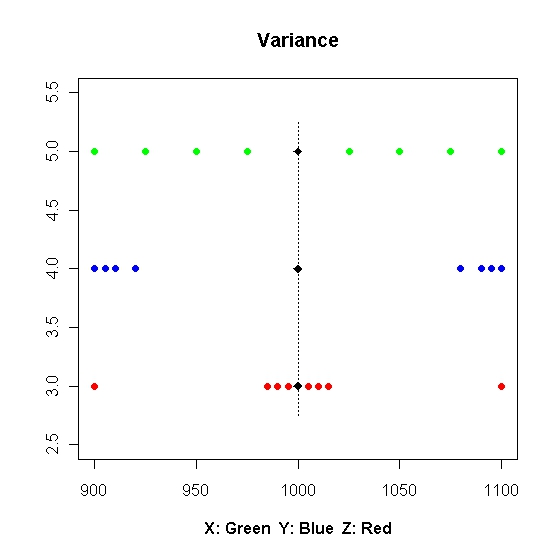
\includegraphics[scale=0.4]{images/images/2AVariance}
\end{center}

}

%--------------------------------------------------------%
{
	{Variance}


\begin{itemize}

\item The (population) variance of a data set is a non-negative number which gives an idea of how widely spread that the population of values are likely to be; the larger the variance, the more scattered the observations on average.
\smallskip
\item Stating the variance gives an impression of how closely concentrated round the expected value the distribution is; it is a measure of the 'spread' of a distribution about its average value.
\smallskip
\item We distinguish between population variance (denoted $\sigma^2$) and sample variance (denoted $s^2$). 
\item For now, we will look only at sample variance.

\end{itemize}

}


%-------------------------------------------------------------------------%
{

	{Sample Variance}

\begin{itemize}

\item Sample variance is a measure of the spread of or dispersion within a set of sample data.
\smallskip
\item The sample variance is the sum of the squared deviations from their mean divided by one less than the number of observations in the data set.
\smallskip
\item For example, for $n$ observations $x_1, x_2, x_3, \ldots , x_n$  with sample mean $\bar{x}$, the sample variance is given by


 \[ s^2 = { \sum (x-\bar{x})^2  \over n-1}\]




\end{itemize}
}
%--------------------------------------------------%
{
	{Sample Standard Deviation}
\begin{itemize}
\item \t{Important:} Standard deviation is the square root of variance
\smallskip
\item Standard deviation is commonly used in preference to variance because it is denominated in the same units as the mean.
\smallskip
\item For example, if dealing with time units, we could have a variance of something like $25$ \emph{ square minutes }, whereas the equivalent standard deviation is 5 minutes.
\smallskip
\item Population standard deviation is denoted  $\sigma$.
\smallskip
\item Sample standard deviation is denoted $s$.
\end{itemize}
}


{
	{Computing Sample Variance}
We shall use the following formulae to compute the sample variance of each data set (i.e. $s^2_x$, $s^2_y$ and $s^2_z$) respectively.

\[ s^2_x = { \sum (x-\bar{x})^2  \over n-1}\]
\[ s^2_y = { \sum (y-\bar{y})^2  \over n-1}\]
\[ s^2_z = { \sum (z-\bar{z})^2  \over n-1}\]
\begin{itemize}
\item Mean for each is 1000: $\bar{x} = \bar{y} = \bar{z}  = 1000$
\item Sample size of each data set is 8 : $ n=8 $
\item Therefore $ n-1 = 7$
\end{itemize}
}
%--------------------------------------------------%
{
	{Computing Sample Variance}
\small
\[ s^2_x = {(900-1000)^2 +(925-1000)^2+ \ldots \ldots +(1075-1000)^2+(1100-1000)^2   \over 7}\]

\[ s^2_x = {(-100)^2 +(-75)^2 +(-50)^2+(-25)^2 + (25)^2 +(50)^2 +(75)^2+(100)^2   \over 7}\]

\[ s^2_x = {37500 \over 7}  = 5357.143\]

\normalsize
\bigskip The sample variance of $X$ is $5357.14$ square units. Recall that the sample standard deviation ($s$) is the square root of the variance, so for $X$  the sample standard deviation is $s_x = 73.19$ units.

}

%--------------------------------------------------%
{
	{Computing Sample Variance}
Similarly \small
\[ s^2_y = {67050 \over 7}  = 9578.571 \mbox{ square units} \]

\[ s^2_z = {20700  \over 7} = 2957.143 \mbox{ square units} \]


\normalsize
\bigskip The sample standard deviations for $Y$ and $Z$ are $s_y = 97.87$ units, and $s_z =  54.38$ units respectively.
}



%----------------------------------------------------------%#